% !Mode:: "TeX:UTF-8"

\chapter{概率分布}
\section{Gamma 函数和Gamma 分布}
Gamma函数的定义为:
\begin{displaymath}
\begin{split}
\Gamma(x)=\int_{0}^{\infty}{u^{x-1}e^{-u}du}
\end{split}
\end{displaymath}
Gama函数的性质:
$\Gamma(1)=1; \Gamma(x+1)=x\Gamma(x); \Gamma(x+1) = x!; \Gamma(\frac{1}{2}) = \sqrt{\pi}$
其中, $\alpha$为形状参数,而$\beta$为尺度参数。

Gamma分布:
\begin{displaymath}
\begin{split}
Gamma(x) = \frac{x^{(\alpha-1)} \lambda^\alpha e^{(-\lambda x)}}{\Gamma(\alpha)}, x > 0
\end{split}
\end{displaymath}

\begin{figure}[htbp]
\centering
\begin{subfloat}
\centering
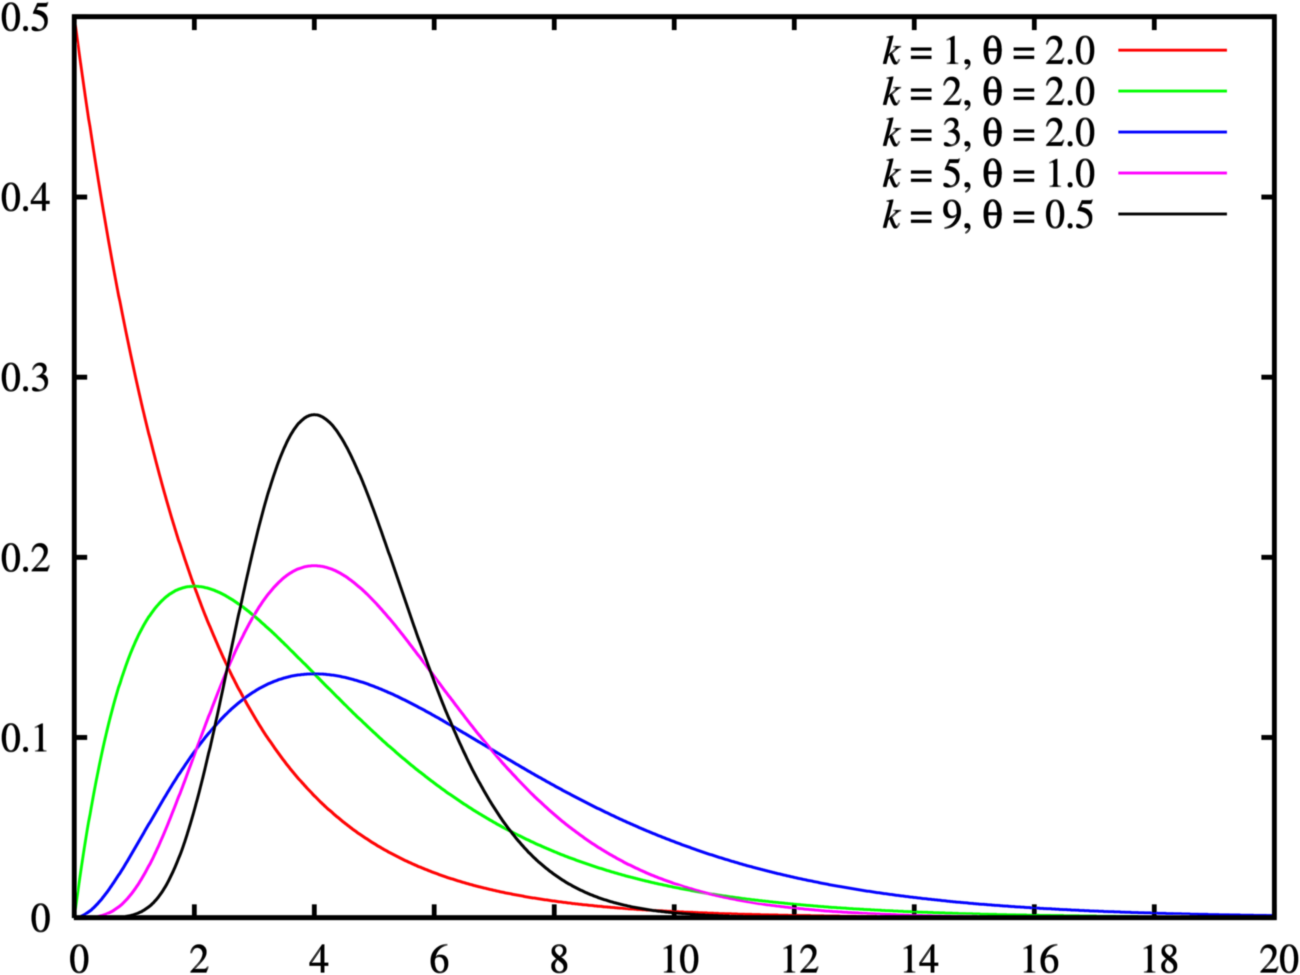
\includegraphics[width = 0.4\textwidth]{figures/Gamma_distribution_pdf.jpg}
\end{subfloat}
\begin{subfloat}
\centering
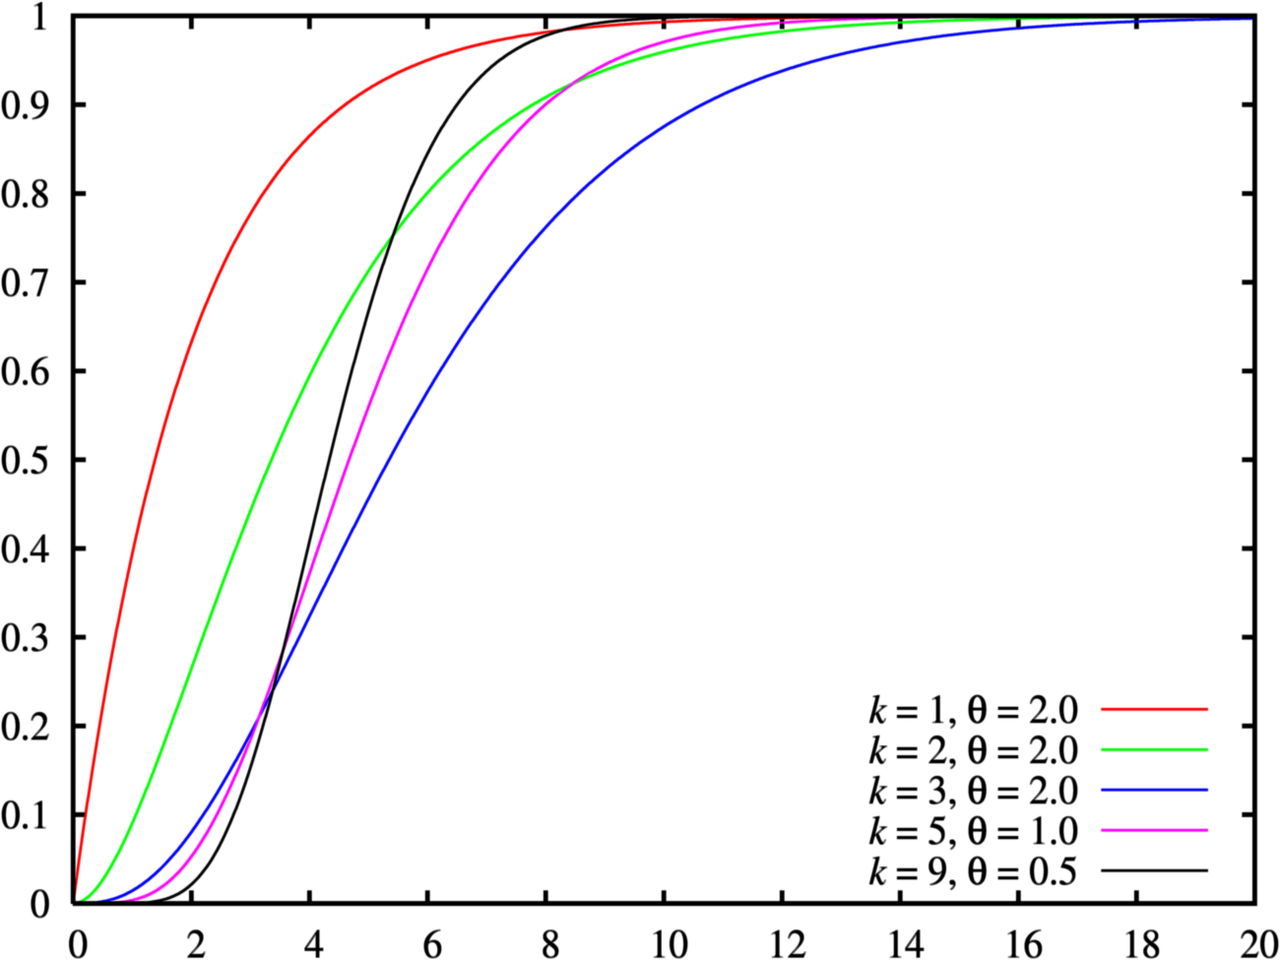
\includegraphics[width = 0.4\textwidth]{figures/Gamma_distribution_cdf.jpg}
\end{subfloat}
\caption{Gamma Distribution}
\end{figure}

参考《Numerical Recipes》第7章,我们有从Gamma分布采样的算法如下:

\begin{minipage}{0.8\textwidth}\centering
\begin{algorithm}[H]
\textbf{Sample from Gamma Distribution}($x \sim Gamma(\alpha, \beta)$):\\
\If{$\alpha < 1$}{
sample $u \sim U(0,1)$;\\
sample $g \sim Gamma(1+\alpha, \beta)$;\\
return $gu^{\frac{1}{\alpha}}$;\\
}
$d=\alpha - \frac{1}{3}, c=\frac{1}{\sqrt{9d}}$;\\
\While{true}{
$v=-1$;\\
\While{$v <= 0$}
{
sample $x \sim N(0,1)$;\\
$v=1+cx$;\\
}
$v = v^3$;\\
sample $u \sim U(0,1)$;\\
\If{$u < 1-0.331x^4$}{
return $\frac{dv}{\beta}$;\\
}
\If{$\ln{u} < 0.5x^2 + d(1-v+\ln{v})$}{
return $\frac{dv}{\beta}$;\\
}

}
\end{algorithm}
\end{minipage}

\begin{figure}[htbp]
\centering
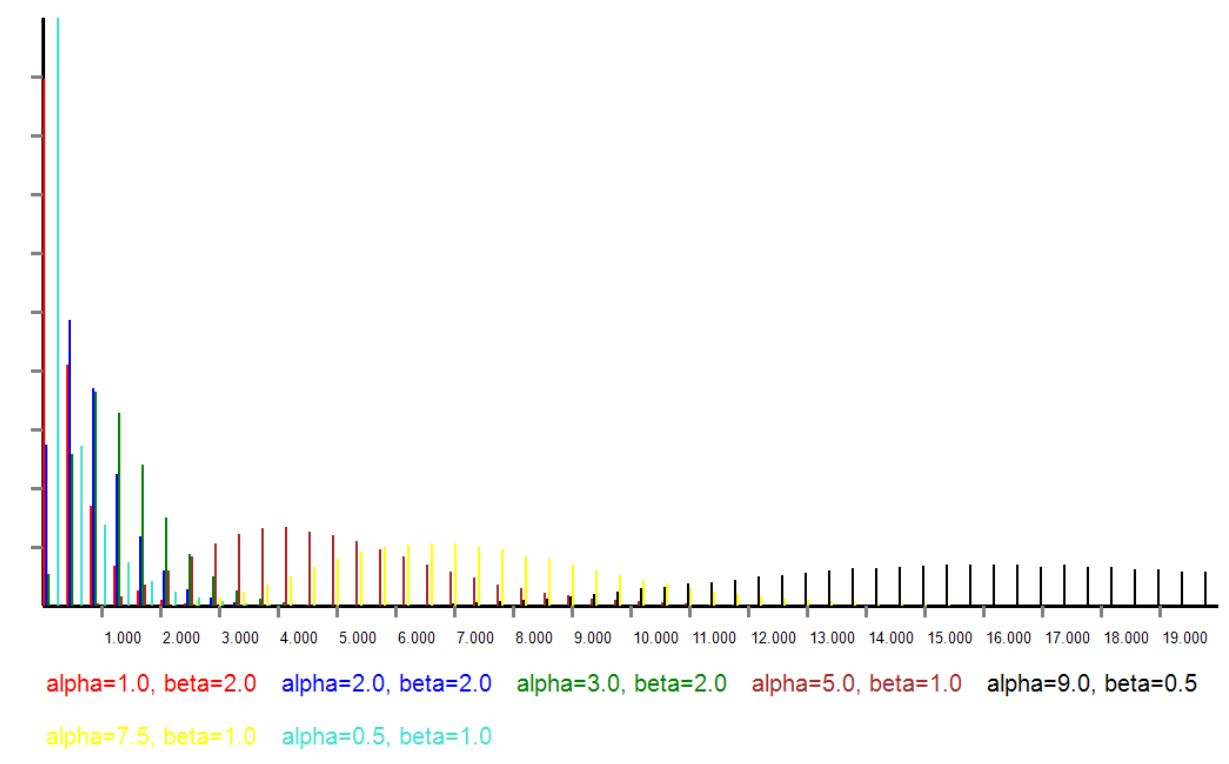
\includegraphics[width = 0.9\textwidth]{GammaDistributionSample}
\caption{从Gamma分布中进行采样}
\end{figure}

\section{Beta-Binomial共轭}

\begin{displaymath}
\begin{split}
Beta(\mu|a,b) &= \frac{\Gamma(a+b)}{\Gamma(a)\Gamma(b)} \mu^{a-1} (1-\mu)^{b-1}\\
Bin(k|\mu, n)  &= \frac{n!}{k!(n-k)!} \mu^k(1-\mu)^{n-k}\\
\end{split}
\end{displaymath}

\begin{displaymath}
\begin{split}
p(\mu|n,k,a,b) &=\frac{Beta(\mu|a,b)Bin(k|\mu,n)}{p(k|n,a,b)}\\
&=\frac{
 \frac{\Gamma(a+b)}{\Gamma(a)\Gamma(b)} \mu^{a-1} (1-\mu)^{b-1} \frac{n!}{k!(n-k)!} \mu^k(1-\mu)^{n-k}
}{
\int_\mu \frac{\Gamma(a+b)}{\Gamma(a)\Gamma(b)} \mu^{a-1} (1-\mu)^{b-1} \frac{n!}{k!(n-k)!} \mu^k(1-\mu)^{n-k} \mathrm{d} \mu
} \\
&= \frac{
 \frac{(a+b-1)! n!}{(a-1)!(b-1)!k!(n-k)!} \mu^{k+a-1} (1-\mu)^{n-k+b-1}
}{
\int_\mu  \frac{(a+b-1)! n!}{(a-1)!(b-1)!k!(n-k)!} \mu^{k+a-1} (1-\mu)^{n-k+b-1} \mathrm{d} \mu
}\\
&= \frac{
 \mu^{k+a-1} (1-\mu)^{n-k+b-1}
}{
\int_0^1 \mu^{k+a-1} (1-\mu)^{n-k+b-1} \mathrm{d} \mu
}\\
&= \frac{
 \mu^{k+a-1} (1-\mu)^{n-k+b-1}
}{
\frac{\Gamma{(k+a)}\Gamma{(n+b-k)}}{\Gamma{(n+a+b)}}
}\\
&= Beta(\mu|a+k, b+n-k)\\
\end{split}
\end{displaymath}
其中:
\begin{displaymath}
\begin{split}
f(0,n) &= \frac{1}{n+1}\\
f(k,n) &= \int_0^1 p^{k}(1-p)^{n-k} \mathrm{d} p\\
&= -p^{k}\frac{(1-p)^{n-(k-1)}}{n-(k-1)} \Bigg |_0^1 + \int_0^1 kp^{k-1} \frac{(1-p)^{n-(k-1)}}{n-(k-1)} \mathrm{d} p\\
& =\int_0^1 kp^{k-1} \frac{(1-p)^{n-(k-1)}}{n-(k-1)} \mathrm{d} p\\
&= \frac{k}{n-(k-1)} \int_0^1 p^{k-1} {(1-p)^{n-(k-1)}} \mathrm{d} p\\
&= \frac{k}{n-(k-1)} f(k-1,n)\\
&= \frac{k(k-1)}{(n-(k-1))(n-(k-2))} f(k-2,n)\\
&= \frac{k(k-1)...1}{(n-(k-1))(n-(k-2))...n} f(0,n)\\
&= \frac{k(k-1)...1}{(n-(k-1))(n-(k-2))...n(n+1)}\\
&= \frac{k!}{\frac{(n+1)!}{(n-k)!}}\\
&= \frac{k!(n-k)!}{(n+1)!}\\
&= \frac{\Gamma(k+1)\Gamma(n-k+1)} {\Gamma(n+2)}\\
\end{split}
\end{displaymath}
另一种证明:
\begin{displaymath}
\begin{split}
&\int_0^1 \frac{\Gamma(n+2)}{\Gamma(k+1)\Gamma(n-k+1)} p^{k}(1-p)^{n-k} \mathrm{d} p = 1\\
\to & \frac{\Gamma(n+2)}{\Gamma(k+1)\Gamma(n-k+1)}  \int_0^1  p^{k}(1-p)^{n-k} \mathrm{d} p = 1\\
\to & \int_0^1  p^{k}(1-p)^{n-k} \mathrm{d} p =  \frac{\Gamma(k+1)\Gamma(n-k+1)} {\Gamma(n+2)} \\
\end{split}
\end{displaymath}
由此:
\begin{displaymath}
\begin{split}
\int_0^1 \mu^{k+a-1} (1-\mu)^{n-k+b-1} \mathrm{d} \mu 
&= \int_0^1 \mu^{k+a-1} (1-\mu)^{(n+a+b-2)-(k+a-1)} \mathrm{d} \mu \\
&= \frac{(k+a-1)!(n+b-k-1)!}{(n+a+b-1)!}\\
&= \frac{\Gamma{(k+a)}\Gamma{(n+b-k)}}{\Gamma{(n+a+b)}}
\end{split}
\end{displaymath}

\begin{figure}[htbp]
\centering
\begin{subfloat}
\centering
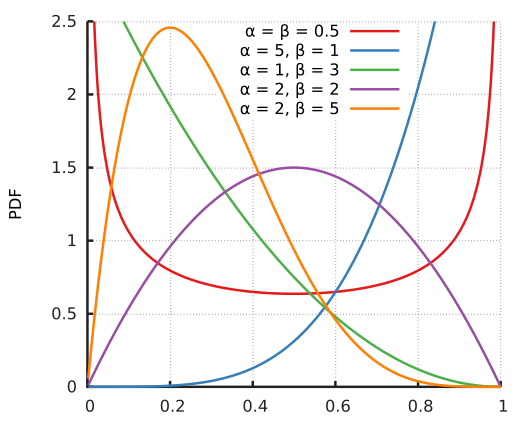
\includegraphics[width = 0.4\textwidth]{Beta_distribution_pdf}
\end{subfloat}
\begin{subfloat}
\centering
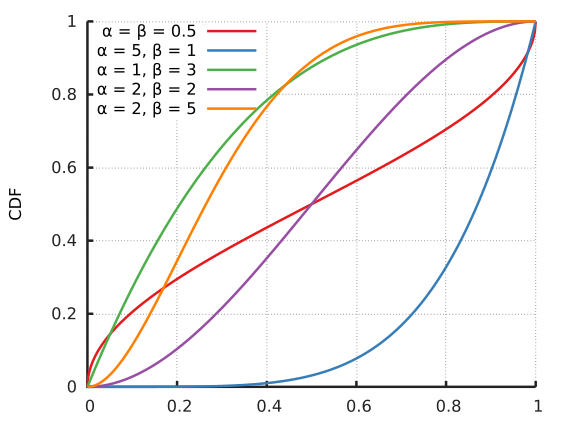
\includegraphics[width = 0.4\textwidth]{Beta_distribution_cdf}
\end{subfloat}
\caption{Beta Distribution}
\end{figure}

使用Gamma分布进行Beta分布采样的算法为:

\begin{minipage}{0.8\textwidth}\centering
\begin{algorithm}[H]
\textbf{Sample from Beta Distribution}($x \sim Beta(\alpha, \beta)$):\\
sample $x_0 \sim Gammma(\alpha, 1)$;\\
sample $x_1 \sim Gamma(\beta, 1)$;\\
return $\frac{x_0}{x_0+x_1}$;\\
\end{algorithm}
\end{minipage}

\begin{figure}[htbp]
\centering
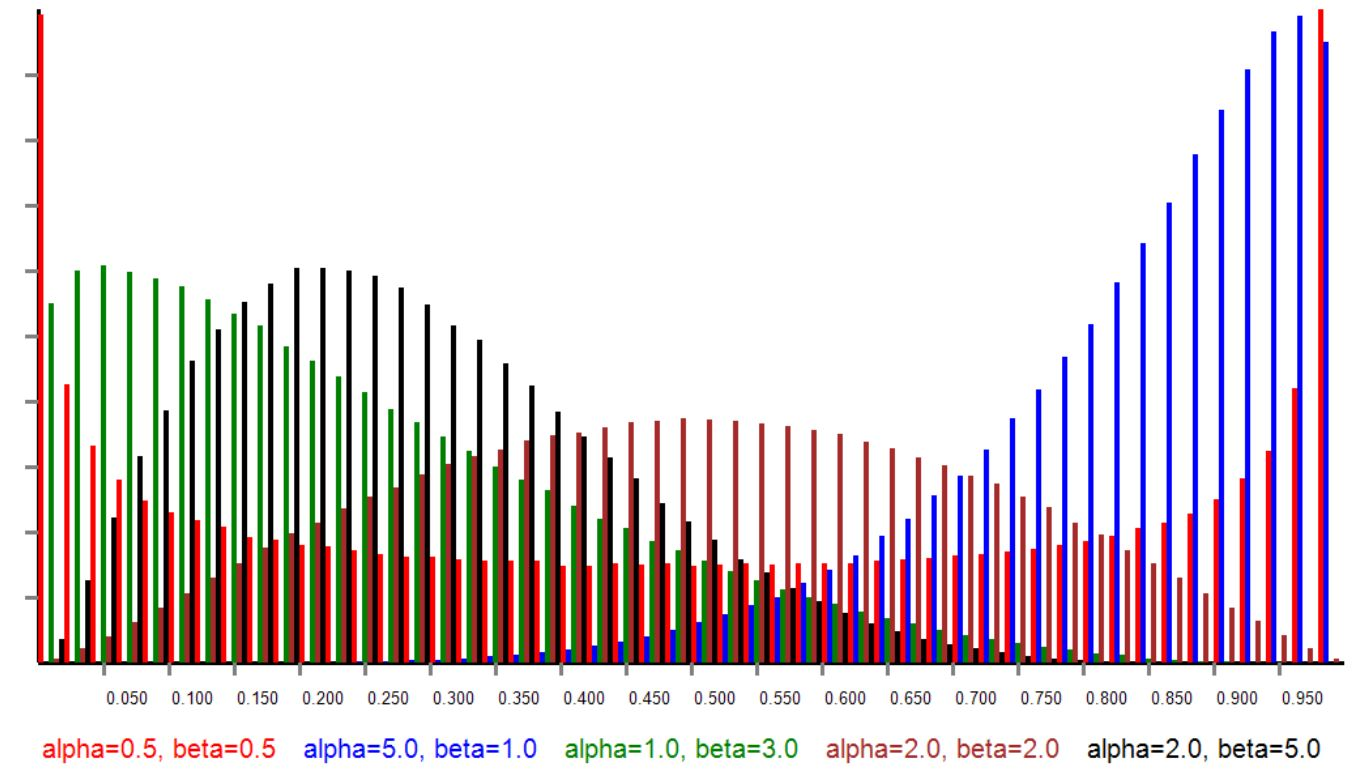
\includegraphics[width = 0.9\textwidth]{BetaDistributionSample}
\caption{从Beta分布中进行采样}
\end{figure}

\section{Dirichlet-Multinomial共轭}
给定数据集$C={c_1,c_2,...,c_n}$,$K$个不同类型出现的次数向量$\vec{N}=(n_1,n_2,...,n_K)$,以及每个类型出现概率的向量$\vec{\pi}=(\pi_0, \pi_1,...,\pi_K)$,其多项式分布的条件概率为:
\begin{displaymath}
p(C|\vec{\pi}) =p(\vec{N}|\vec{\pi})= \prod_{k=1}^{K}\pi_k^{n_k}
\end{displaymath}
参数为$\vec{A} = (a_1,a_2...a_K)$的Dirichlet分布的定义如下:
\begin{displaymath}
\begin{split}
Dir(\vec{\pi}|\vec{A})=\frac{\Gamma{(\sum_{k=1}^{K}{a_k}})}{\prod_{k=1}^{K}{\Gamma{(a_k)}}}\prod_{k=1}^{K}{\pi_{k}^{a_k-1}}
\end{split}
\end{displaymath}
当Dirichlet分布作为多项式分布的先验分布式时,其后验分布为:
\begin{displaymath}
\begin{split}
p(C|\vec{A},\vec{N})
&= \frac{p(\vec{N}|\vec{\pi}) p(\vec{\pi}|\vec{A})}{\int_{\vec{\pi}} p(\vec{M}|\vec{\pi}) p(\vec{\pi}|\vec{A})  \mathrm{d} \vec{\pi}}\\
&= \frac{
\frac{\Gamma{(\sum_{k=1}^{K}{a_k}})}{\prod_{k=1}^{K}{\Gamma{(a_k)}}}\prod_{k=1}^{K}{\pi_{k}^{a_k-1}} \prod_{k=1}^{K}\pi_k^{n_k} 
}{ \int_{\vec{\pi}}
\frac{\Gamma{(\sum_{k=1}^{K}{a_k}})}{\prod_{k=1}^{K}{\Gamma{(a_k)}}}\prod_{k=1}^{K}{\pi_{k}^{a_k-1}} \prod_{k=1}^{K}\pi_k^{n_k}   \mathrm{d} \vec{\pi}
}\\
&= \frac{
\prod_{k=1}^{K}{\pi_{k}^{a_k+n_k-1}}
}{ \int_{\vec{\pi}}
\prod_{k=1}^{K}{\pi_{k}^{a_k+n_k-1}}   \mathrm{d} \vec{\pi}
}
= \frac{
\prod_{k=1}^{K}{\pi_{k}^{a_k+n_k-1}}
}{ 
\frac{\prod_{k=1}^{K} \Gamma(a_k+n_k)}{\Gamma(\sum_{k=1}^K(a_k+n_k))}
}\\
&= \frac{\Gamma{(\sum_{k=1}^{K}{(a_k+n_k)}})}{\prod_{k=1}^{K}{\Gamma{(a_k+n_k)}}}\prod_{k=1}^{K}{\pi_{k}^{a_k+n_k-1}}\\
&= Dir(\vec{\pi}|\vec{A}+\vec{N})\\
\end{split}
\end{displaymath}
即:给定一个Dirichlet分布的先验和一个多项式分布的条件概率,可以得到一
个Dirichlet分布的一个后验。

\begin{displaymath}
\begin{split}
&\int_{\vec{\pi}} \frac{\Gamma{(\sum_{k=1}^{K}{a_k}})}{\prod_{k=1}^{K}{\Gamma{(a_k)}}}  \prod_{k=1}^{K}{\pi_{k}^{a_k-1}}   \mathrm{d} \vec{\pi} =1 \\
\to & \frac{\Gamma{(\sum_{k=1}^{K}{a_k}})}{\prod_{k=1}^{K}{\Gamma{(a_k)}}} \int_{\vec{\pi}}  \prod_{k=1}^{K}{\pi_{k}^{a_k-1}}   \mathrm{d} \vec{\pi} =1 \\
\to &  \int_{\vec{\pi}}  \prod_{k=1}^{K}{\pi_{k}^{a_k-1}}   \mathrm{d} \vec{\pi} =  \frac{\prod_{k=1}^{K}{\Gamma{(a_k)}}}  {\Gamma{(\sum_{k=1}^{K}{a_k}})}\\
\end{split}
\end{displaymath}


\begin{figure}[htbp]
\centering
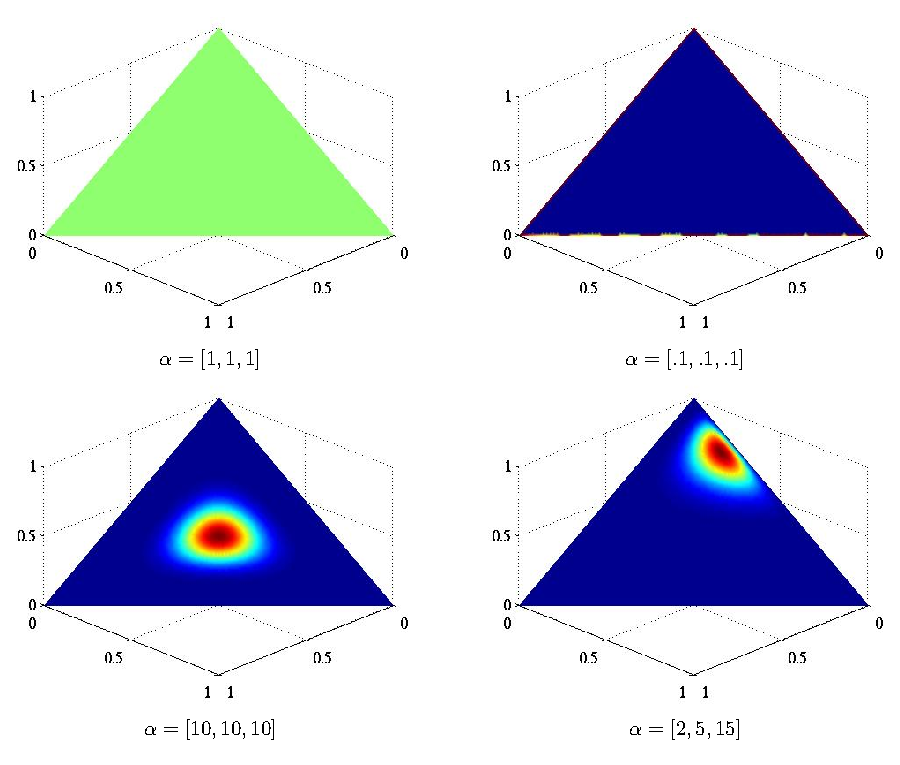
\includegraphics[width = 0.8\textwidth]{DirichletDistribution}
\caption{Dirichlet Distribution}
\end{figure}

对于一个对称的狄利克雷分布
\begin{displaymath}
\begin{split}
p(\pi_1,...,\pi_k|a)&=Dir(a/k, ... ,a/k) = \frac{\Gamma{(a)}}{{\Gamma{(a/k)}}^k} \prod_{j=1}^{k}{\pi_{j}^{a/k-1}}\\
p(C|a) &= \frac{\Gamma{a}}{\Gamma(a/k)^k} \int \prod_{j=1}^{k} \pi_j^{n_j+a/k-1} \mathrm{d} \pi_j\\
&= \frac{\Gamma{(a)}}{\Gamma(a/k)^k} \frac{\prod_{j=1}^{k}{\Gamma{(a/k +n_j)}}}  {\Gamma{(a + n)}}\\
&= \frac{\Gamma{(a)}}{\Gamma(a+n)} \prod_{j=1}^{k} \frac{\Gamma{(a/k +n_j)}} {\Gamma{(a/k)}}\\
\end{split}
\end{displaymath}

则:
\begin{displaymath}
\begin{split}
p(c_i=j|\mathbf{c}_{-i},a) &= \frac{p(\mathbf{c}|a)}{p(\mathbf{c}_{-i}|a)}\\
&= \frac{ \frac{\Gamma{(a)}}{\Gamma(a+n)} \prod_{j=1}^{k} \frac{\Gamma{(a/k +n_j)}} {\Gamma{(a/k)}}
}{\frac{\Gamma{(a)}}{\Gamma(a+n-1)}  \frac{\Gamma{(a/k +n_{j, -i})}} {\Gamma{(a/k)}} \prod_{j' \neq j} \frac{\Gamma{(a/k +n_{j'})}} {\Gamma{(a/k)}}
}\\
&= \frac{\Gamma{(n+a-1)}}{\Gamma(a+n)} \frac{\frac{\Gamma{(a/k +n_{j})}} {\Gamma{(a/k)}}}{\frac{\Gamma{(a/k +n_{j, -i})}} {\Gamma{(a/k)}}}\\
&= \frac{\Gamma{(n+a-1)}}{\Gamma(a+n)} \frac{\Gamma{(a/k +n_{j})}} {\Gamma{(a/k +n_{j, -i})}} \\
&= \frac{\Gamma{(n+a-1)}}{\Gamma(a+n)} \frac{\Gamma{(a/k +n_{j, -i} +1)}} {\Gamma{(a/k +n_{j, -i})}} \\
&= \frac{n_{j, -i} + a/k}{n+a-1}\\
\end{split}
\end{displaymath}


\subsection{Sample from Dirichlet Distribution}

如何从参数为$\vec{A} = (a_1,a_2...a_K)$的Dirichlet分布$Dir(\vec{\pi}|\vec{A})$中采样一个$\vec{\pi}$呢?

\textbf{Polya's Urn}
 
我们首先介绍一种简单的方法,即Polya's Urn。
如图所示,我们首先在一个桶中放入$K$种颜色的球各$\vec{A} = (a_1,a_2...a_K)$个,然后我们随机的从桶中拿一个球,并额外拿一个同样颜色的球,一并放回桶中,我们一直重复这个过程,可以证明,当这个操作趋向于无穷次时,桶里的球的分布将逼近一个从狄利克雷分布上的一个采样。

\begin{figure}[htbp]
\centering
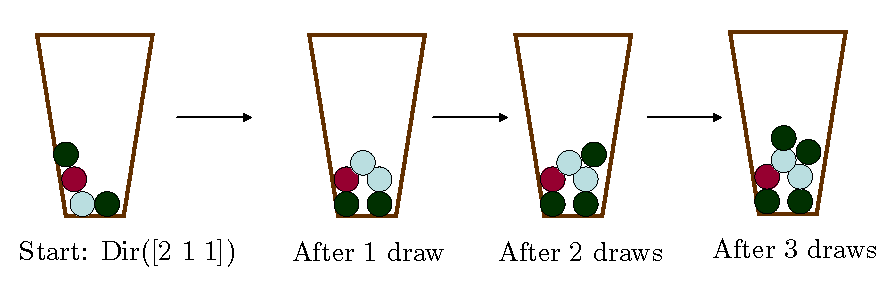
\includegraphics[width = 0.8\textwidth]{Urn-Drawing}
\end{figure}

\textbf{Stick-Breaking}

我们先来说$K=3$的情况,即 $\vec{A} = (a_1,a_2,a_3)$。我们首先从Beta分布$Beta(a_1, a_2+a_3)$中采样一个值$u_1$,并进一步的从Beta分布$Beta(a_2,a_3)$中采样一个值$u_2$,那么$(u_1, (1-u_1)u_2, 1-u_1-(1-u_1)u_2)$便是狄利克雷分布$Dir(\vec{\pi}|(a_1,a_2,a_3))$的一个采样。

\begin{figure}[htbp]
\centering
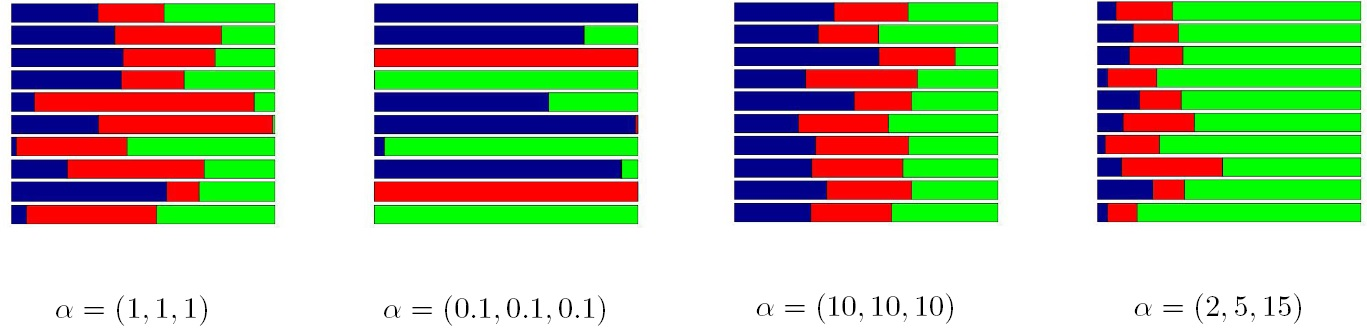
\includegraphics[width = 1.0\textwidth]{StickBreaking}
\end{figure}

当$K>3$时,我们首先从Beta分布$Beta(a_1, \sum_{2}^{k}a_k)$中采样一个值$u_1$,则剩余的棍的长度为$1-u_1$。对于$1<j<k$,如果长度$u_1,u_2,...,u_{j-1}$已经产生,则剩余棍的长度为:$\prod_{i=1}^{j-1}(1-u_i)$,我们从Beta分布$Beta(a_j, \sum_{i=j+1}^{k}a_i)$中采样一个$u_j$,并令$q_j=u_j\prod_{i=1}^{j-1}(1-u_i)$,则剩余的长度为$\prod_{i=1}^{j-1}(1-u_i) - u_j\prod_{i=1}^{j-1}(1-u_i) = \prod_{i=1}^{j}(1-u_i)$。令剩余长度为$q_k$,则$(q_1. q_2,...,q_k)$是狄利克雷分布$Dir(\vec{\pi}|(a_1,a_2,...,a_k))$的一个采样。

\begin{figure}[htbp]
\centering
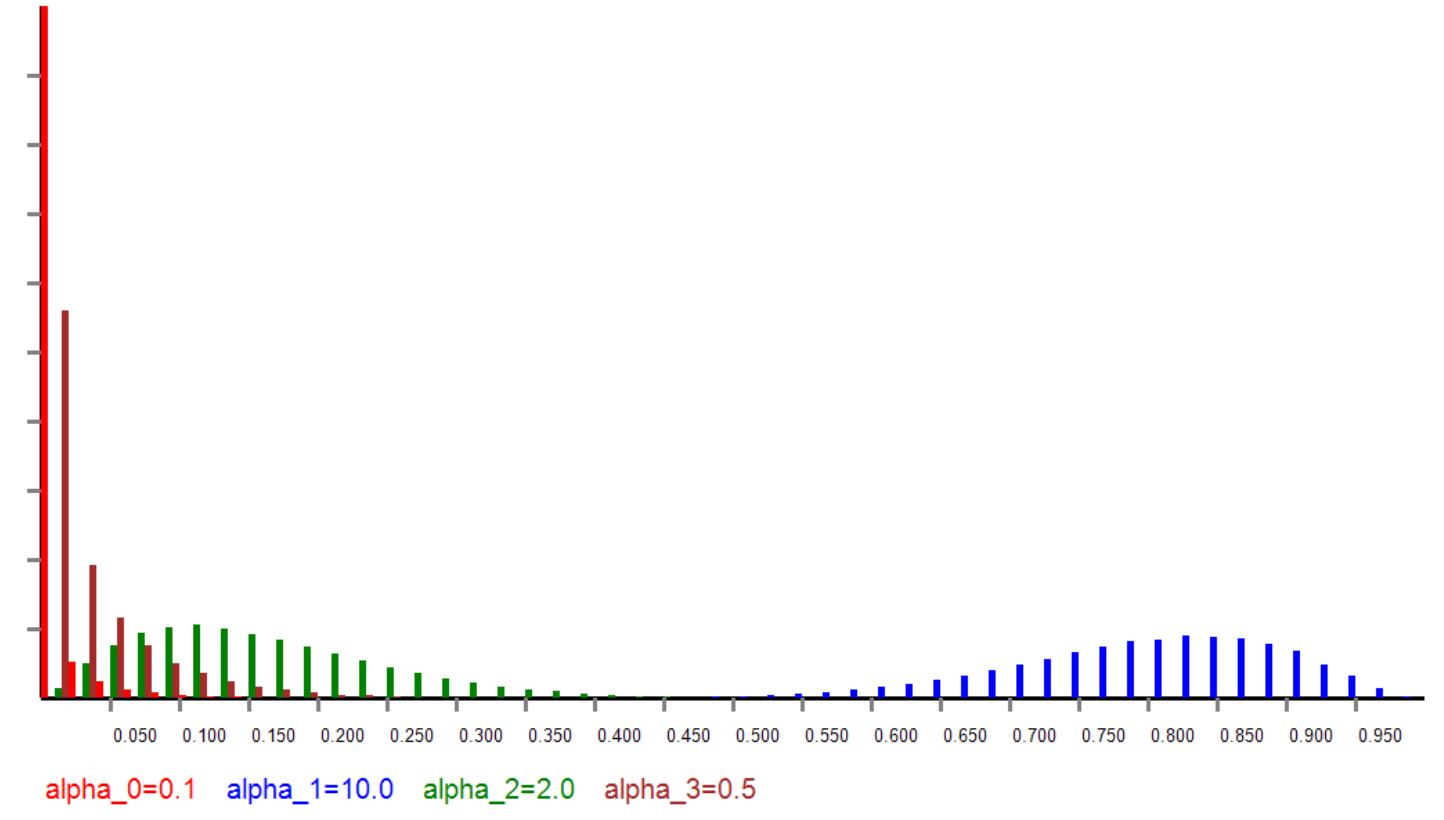
\includegraphics[width = 0.9\textwidth]{DirichletDistributionSample}
\caption{从Dirichlet分布中进行采样}
\end{figure}